\chapter{Processi stocastici}

\begin{figure}[h]
    \centering
    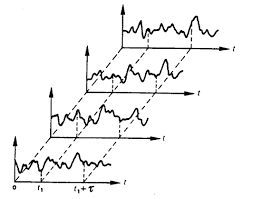
\includegraphics[scale = 1.5]{Processo stocastico.png}
\end{figure}   

\newpage 

\section{Processi stocastici: cosa sono}

I segnali aleatori vengono comunemente denominati processi stocastici. \newline 

Per un processo stocastico non è definibile, e dunque calcolabile, la trasformata di Fourier perchè 
la trasformata di Forurier presuppone la conoscenza dell'andamento del segnale. \newline 

L'evoluzione di un processo stocastico può essere descritto solo statisticamente. \newline 

Piuttosto che usare come dominio la frequenza e la trasformata di Forurier, 
per un processo stocastico si sceglierà di utilizzare lo spettro di potenza del processo. \newline 

Consideriamo la seguente figura: 

\begin{figure}[h]
    \centering
    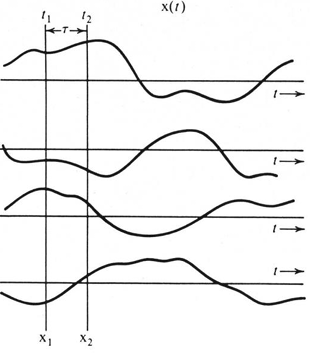
\includegraphics[scale = 1]{Processo stocastico segnali.PNG}
\end{figure}  

Tutti questi andamenti sono di un processo stocastico x(t). \newline 

Al fine di descrivere statisticamente il processo, si può fissare l'attenzione sul valore assunto da x(t) in un generico istante (ad esempio $t_1$) 
e valutare la densità di probabilità $f_1 (x_1; t_1)$ della variabile aleatoria estratta $x_1 = x(t_1)$. \newline 

Allo steso modo si può considerare un altro istante $t_2$ e valutare la corrispondente $f_2 (x_2; t_2)$, 
che in questo caso rappresenterà la densità di probabilità della variabile aleatoria estratta $x_2 = x(t_2)$. \newline 

La procedura può essere estesa ad un numero arbitrario di istanti (e quindi di variabili aleatorie estratte). \newline 

Una descrizione più accurata si ottiene prendendo in esame, contemporaneamente, due istanti generici (ad esempio $t_1$ e $t_2$) e valutando la densità di probabilità congiunta $f_{12} (x_1, x_2; t_1, t_2)$. \newline 

La probabilità congiunta $f_{12} (x_1, x_2; t_1, t_2)$ molte delle volte è una soluzione alla maggior parte dei problemi. \newline 


\newpage 

\section{Medie di insieme} 

Per le variabili aleatorie estratte dal processo sono calcolabili le medie di insieme. \newline 

Consideriamo il valore medio in $x_1$, che sarà dato da: 

{
    \Large 
    \begin{equation}
        <x_1> 
        = 
        \int_{- \infty}^{+\infty}
        x_1 f_1 (x_1; t_1) dx_1
    \end{equation}
}

Il momento congiunto di ordine (1, 1) delle variabili $x_1$ e $x_2$ si otterrà come: 

{
    \Large 
    \begin{equation}
        <x_1 x_2> 
        = 
        \int_{- \infty}^{+\infty}
        \int_{- \infty}^{+\infty}
        x_1 x_2 f_{12} (x_1, x_2; t_1, t_2) 
        dx_1
        dx_2
    \end{equation}
}

Il momento congiunto di ordine (1, 1), che rappresenta la correlazione tra le variabili aleatorie estratte $x_1$ e $x_2$; 
prende il nome di autocorrelazione statistica del processo e si indica con $R(t_1, t_2)$. \newline 

Si noti che nelle densità di probabilità, in $<x_1>$ e $<x_1 x_2>$ le variabili aleatorie sono le $x_i$ mentre il tempo svolge il ruolo di paramentro. \newline 

In generale, le densità di primo ordine sono diverse al variare dell'istante $t_i$ considerato e le densità di ordine superiore 
dipendono singolarmente dagli istanti $t_i, t_j, ..., t_k$. \newline 

Più frequentemente, si può ritenere vera la circostanza che una traslazione arbitraria dall'origine dei tempi dell'intero 
processo non ne modifichi le caratteristiche statistiche. \newline 


\newpage 
\section{Stazionarietà e ergodicità}
Con riferimento alle definizioni precedenti, ciò comporta che: 

\begin{itemize}
    \item la densità del primo ordine è indipendete da t, ed è quindi la stessa per ogni possibile variabile aleatoria estratta 
    \item la densità del secondo ordine dipende solo dalla differenza $\tau = t_2 - t_1$
    \item la densità di probabilità di ordine n dipende solo dagli $n-1$ parametri
\end{itemize}

Un processo di questo tipo si dice stazionario in senso stretto e, per esso, la densità di probabilità del 
primo e del secondo ordine si scrivono $f(x)$ e $f_{12} (x_1, x_2; \tau)$ rispettivamente. \newline 

Accanto alla stazionarietà in senso stretto, si può definire anche la stazionarietà in senso lato. \newline 

Si può defnire un processo con stazionarietà in senso lato se ha valore medio $<x_1>$ è indipendente da t e la cui 
autocorrelazione statistica $<x_1 x_2>$ dipende solo dalla differenza $\tau = t_2 - t_1$. \newline 

La stazionarietà in senso stretto implica, ovviamente, la stazionarietà, mentre non è vero il viceversa. \newline 

La proprietà di stazionarietà è propedeutica ad un altro fondamentale concetto: quello di ergodicità. \newline 

In un processo ergodico ogni realizzazione è tipica del processo, nel senso che la sua osservazione per un tempo sufficientemente lungo consente di estrarre tutte le 
proprietà del processo stesso. \newline 

L'accuratezza della stima può essere arbitrariamente migliorata aumentando il livello di risoluzione orizzontale (vale a dire, riducendo l'estensione degli intervalli) 
ed assumendo un valore di N via via più elevato. \newline 

In figura un esempio di intervalli sempre più stretti: 

\begin{figure}[h]
    \centering
    \includegraphics[scale = 0.7]{Intervalli più stretti.PNG}
\end{figure}  


L'istogramma può essere utilizzato per stimare la densità di probabilità del secondo ordine o una qualunque media di insieme. \newline 

Un processo ergodico, in tutte le sue densità di probabilità di qualasiasi ordine, si dirà 
generalmente, ergodico. \newline 

Se le considerazioni qualitative precedenti fossero formalizzate in termini rigorosamente analitici, 
ci saremo resi conto che l'ergodicità presuppone la stazionarietà. \newline 

In altri termini, non può essere ergodico un processo che non è stazionario. \newline 

La maggior parte dei processi reali non sono intriscamente ergodici, ma, possono essere separati e/o ridotti in processi 
più semplici e singolarmente ergodici.\newline 


Per un processo stocastico, possiamo considerare anche le medie temporali. \newline 

Il valore medio temporale di una generica realizzazione del processo x(t) è definito come: 

{
    \Large 
    \begin{equation}
        \overline{x(t)} 
        =
        \lim_{\Delta t \to \infty}
        \frac{1}{\Delta t}
        \int_{-\frac{\Delta t}{2}}^{\frac{\Delta t}{2}} 
        x(t) dt  
    \end{equation}
}

$\overline{x(t)} = <x> $ in parole, possiamo vedere il valore medio temporale come il valore medio statistico. \newline 

Invece, l'autocorrelazione temporale possiamo definirla come: 

{
    \Large 
    \begin{equation}
        \overline{R (\tau)} 
        = 
        \lim_{\Delta t \to \infty}
        \frac{1}{\Delta t}
        \int_{-\frac{\Delta t}{2}}^{\frac{\Delta t}{2}} 
        x(t) 
        x(t + \tau)
        dt  
    \end{equation}
}

in cui $\tau = t_2 - t_1$ e $\overline{x(t)} = <x_1 x_2> $.  \newline 


La generica realizzazione del processo, una volta specificata (vale a dire, misurata o registrata), 
può essere riguardata come un particolare segnale determinato a potenza finita. \newline 

Per esso si può definire una densità spettrale (o semplicemente spettro di potenza) $p(\omega)$ che, 
in accordo con i segnali determinati, sarà data da: 

{
    \Large 
    \begin{equation}
        p(\omega) = \lim_{\Delta t \to \infty} \frac{\abs{X_\Delta (\omega)}^{2}}{\Delta t}
    \end{equation}
}


dove $X_\Delta (\omega)$ è la trasformata di Foruier del segnale che si ottiene considerando x(t) entro un intervallo, 
centrato nell'origine e di estensione $\Delta t$. \newline 

\newpage 

\section{Processo ergodico e il teorema di Wiener-Khintchine}

Nel caso di un processo erogodico, le medie di insieme (vale a dire le medie statistiche) coincidono con le medie temporali e possono essere 
calcolate a partire da un'unica e generica realizzazione del processo. \newline 

Per questo tipo di processi, possiamo enunciare il seguente teorema, il teorema di Wiener-Khintchie: 
se il processo x(t) è stazionario ed ergodico, almeno nella sua autocorrelazione, lo spettro di potenza del processo ad esso associato risulta 
la trasformata di Fourier della sua autocorrelazione statistica $R(\tau)$. \newline 


Sempre in virtù dell'ergodicità e delle proprietà ad esse associate, si può osservare che:

{
    \Large 
    \begin{equation}
        \begin{split}
            P 
            &= 
            \lim_{\Delta t \to \infty}
            \frac{1}{\Delta t}
            \int_{-\frac{\Delta t}{2}}^{\frac{\Delta t}{2}}
            x^{2} (t) dt 
            \\ 
            &= 
            \overline{R (0)}
            \\ 
            &= 
            R(0)
            \\ 
            &= 
            <x_1 ^{2}>
        \end{split}
    \end{equation}
}

Come nel transito di un segnale di potenza determinato attraverso un sistema lineare, 
anche lo spettro di potenza di un processo stocastico ergodico viene alterato come: 

{
    \Large 
    \begin{equation}
        p_y (\omega) = \abs{H (\omega)}^{2} p_x (\omega)
    \end{equation}
}

\newpage 

\section{Teorema di Weiner-Khintchine generalizzato}

Possiamo definire il teorema di Weiner-Khintchine anche per fenomeni non ergodici, che prende il nome del Teorema di Weiner-Khintchine generalizzato. \newline 


Se per ogni valore di $\tau$ e ogni intervallo A di estensione pari a $\abs{\tau}$, la funzione di autocorrelazione del segnale aleatorio x(t) soddisfa la condizione:
{
    \Large 
    \begin{equation}
        \abs{\int_{A} R_X (t+ \tau, t) dt} < \infty
    \end{equation}
}

allora la densità spettrale di potenza di x(t) è la trasformata di Fourier della funzione 
$R_X (t+ \tau, t)$ mediata rispetto a t. \newline 

In formule: 

{
    \Large 
    \begin{equation}
        S_X (f) = F[\lim_{T \to \infty} \frac{1}{T} \int_{- \frac{T}{2}}^{\frac{T}{2}} R_X (t+ \tau, t) dt ]
    \end{equation}
}

dove per $F[\cdot]$ si intende la trasformata di Fourier della funzione all'interno delle parentesi quadrate 
e $S_X (f)$ è la densità spettrale di potenza. \newline 

\newpage 

\section{Segnali ciclostazionari}

Un importante esempio di applicazione del teorema di Wiener-Khintchine generalizzato si ha con i segnali ciclostazionari. \newline 

Si definisce ciclostazionario un segnale aleatorio x(t) il cui valore medio E[x(t)] e la cui funzione di autocorrelazione $R_X (t + \tau, t)$ sono 
funzioni periodiche di periodo comune $T_0$: 

{
    \Large 
    \begin{equation}
        E[x(t + T_0)] = E[x(t)]
    \end{equation}
}

in altre parole, il valore medio è uguale ogni $T_0$, inoltre: 

{
    \Large 
    \begin{equation}
        R_X (t + \tau + T_0, t + T_0) = R_X (t + \tau, t)
    \end{equation}
}

\newpage
. 
\newpage
. 
\newpage